\documentclass[10pt]{beamer}
\usepackage{ragged2e} % \justifying
\usepackage[export]{adjustbox} % left and right in images
\usetheme{metropolis}           % Use metropolis theme
\title{Vision-based Autonomous Landing in Catastrophe-Struck Environments}
\subtitle{\textit{Authors:} Mayank Mittal, Abhinav Valada, Wofram Burgard}
\date{\today}
\author{Michele Cipriano}
\institute{Control Problems in Robotics: Modeling and control of
    multi-rotor UAVs\\Department of Computer, Control and Management
    Engineering\\Sapienza University of Rome}

% Fontsize of figure smaller than normalsize:
\setbeamerfont{caption}{size=\scriptsize}

\begin{document}
\nocite{*}

    \maketitle

    \begin{frame}{Introduction}
            Equipping UAVs with \textbf{bioradars}:
            \begin{itemize}
                \item estimate a set of candidate \textbf{safe landing sites}
                \item optimize over the global area via \textbf{clustering}
                \item project landing sites onto \textbf{volumetric reconstruction}
                \item compute a \textbf{minimum-jerk trajectory} to land
                    on debris piles
                \item validate on simulated and real-world environments
            \end{itemize}
    \end{frame}

%    \begin{frame}{Technical Approach}
%        \begin{columns}[c,onlytextwidth]
%            \column{0.5\textwidth}
%            \begin{itemize}
%                \item State Estimation
%                \item Landing Site Detection
%                \item 3D Volumetric Mapping
%                \item Landing Trajectory Estimation
%            \end{itemize}
%            \column{0.5\textwidth}
%                \begin{figure}
%                    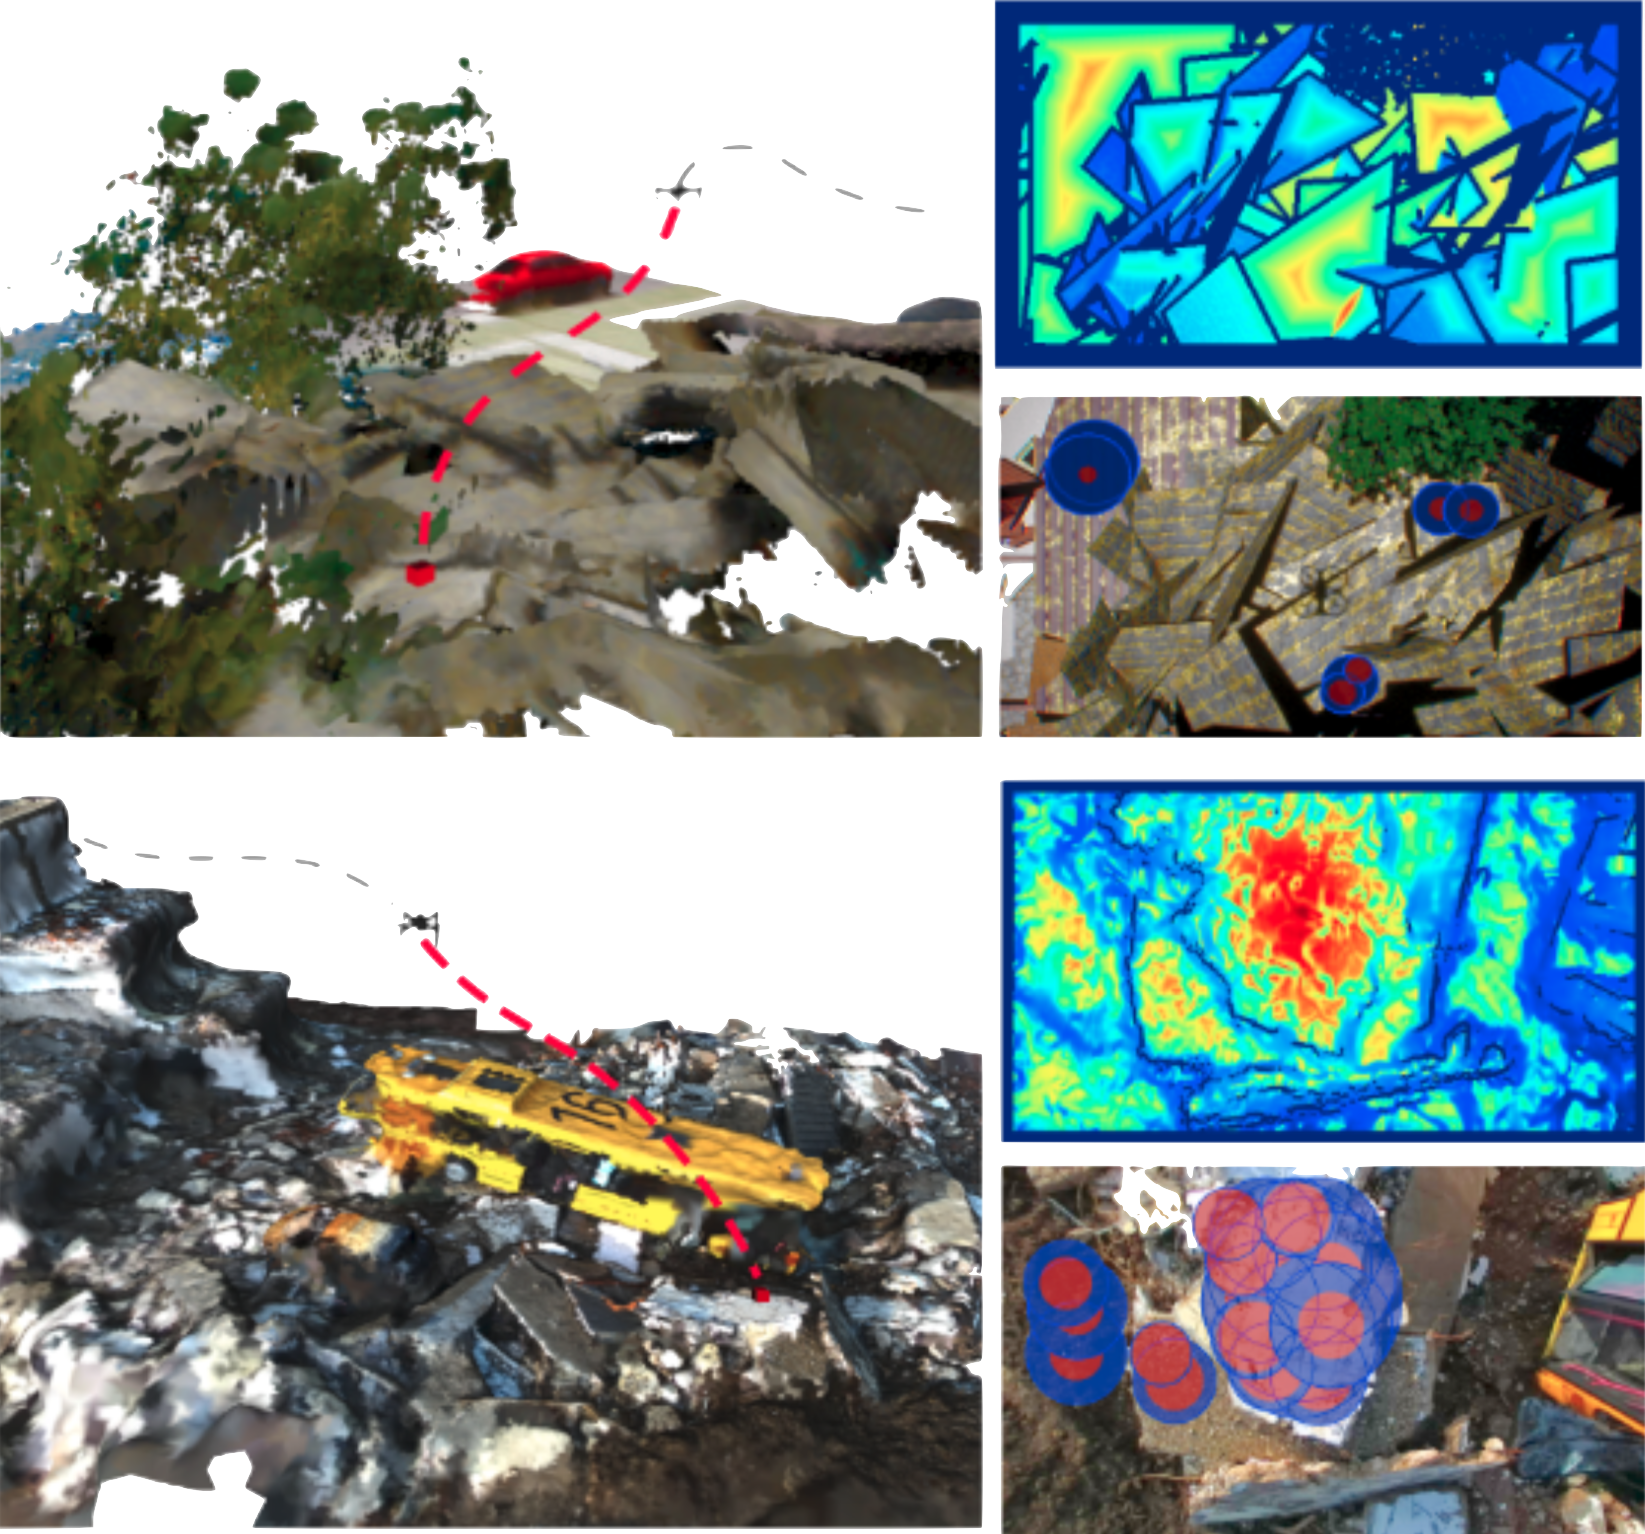
\includegraphics[width=0.96\textwidth,right]{images/Fig1.png}
%                \end{figure}
%        \end{columns}
%    \end{frame}

    \begin{frame}{Technical Approach: State Estimation}
        \justifying
        \begin{itemize}
            \item \textbf{ORB-SLAM2} (oriented FAST and rotated BRIEF)
            \item downward-facing stereo camera
            \item multi-sensor fusion (EKF) using IMU, barometer and GPS
            \item sensors precalibrated with Kalibr toolbox
        \end{itemize}
    \end{frame}

%    \begin{frame}{Technical Approach: Landing Site Detection}
%        \justifying
%        \begin{itemize}
%            \item Depth Information $J_{DE}$
%            \item Flatness Information $J_{FL}$
%            \item Steepness Information $J_{N}$
%            \item Energy Consumption Information $J_{EC}$
%            \item k-d tree + agglomerative hierarchical clustering algorithm
%        \end{itemize}
%    \end{frame}

    \begin{frame}{Technical Approach: Landing Site Detection}
        \begin{columns}[c,onlytextwidth]
            \column{0.57\textwidth}
            \begin{itemize}
                \small
                \item Depth Information $J_{DE}$
                \item Flatness Information $J_{FL}$
                \item Steepness Information $J_{N}$
                \item Energy Consumption Information $J_{EC}$
                \item k-d tree + agglomerative hierarchical clustering algorithm
            \end{itemize}
            \column{0.43\textwidth}
                \begin{figure}
                    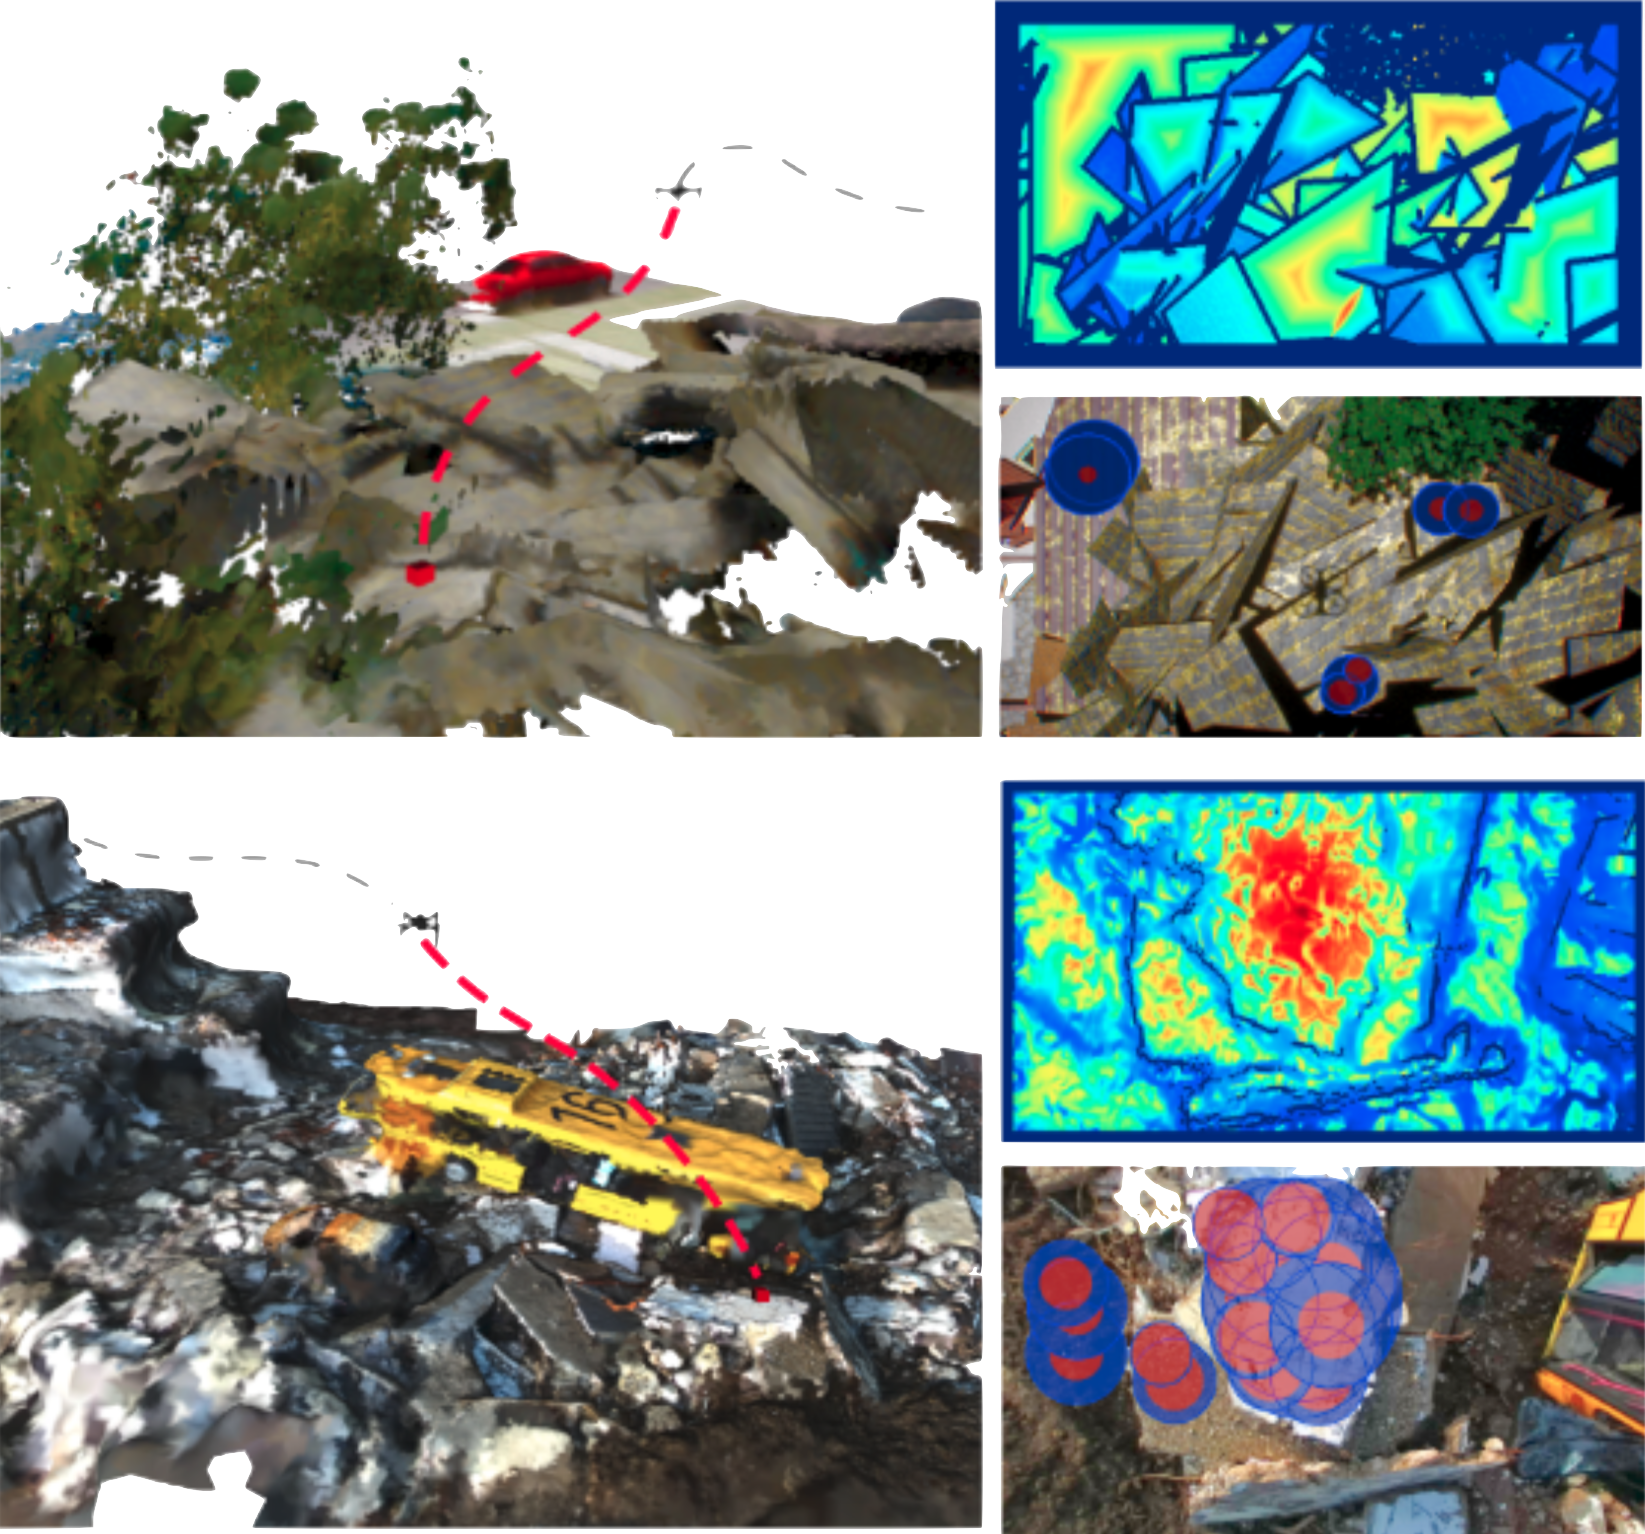
\includegraphics[width=\textwidth]{images/Fig1.png}
                \end{figure}
        \end{columns}
    \end{frame}

    \begin{frame}{Technical Approach: Landing Site Detection}
        \justifying
        Confidence in \textbf{\textsc{Depth Information}} $J_{DE}$:
        \begin{equation*}
            J_{DE}(p) = 1 - \frac{D(p)^2 - min\{D^2\}}{max\{D^2\}}
        \end{equation*}
        with $D$ depthmap obtained from the stereo camera and $p=(x,y)$
        pixel in the depthmap.
    \end{frame}

    \begin{frame}{Technical Approach: Landing Site Detection}
        \justifying
        \textbf{\textsc{Flatness Information}} $J_{FL}$:
        \begin{gather*}
            di(B, p) = min\Big\{\|p-q\| \Big| B(q)=1\Big\} \\
            J_{FL}(p) = di(Canny(D), p)
        \end{gather*}
        with $B$ binary image and $p, q$ pixels in the image plane. $Canny$
        applies the \textbf{Canny edge detector} over the depthmap $D$.
    \end{frame}

    \begin{frame}{Technical Approach: Landing Site Detection}
        \justifying
        \textbf{\textsc{Steepness Information}} $J_{N}$:
        \begin{itemize}
            \item point cloud from the depthmap in global frame
            \item \textbf{average 3D gradients algorithm} to estimate normals map $N$
            \item evaluate deviation of the normalized surface normal
                $\hat{n}$ wrt z-axis $\hat{z}$ in the world frame:
                $\theta = cos^{-1}(\hat{n}^T\hat{z})$
            \item compute steepness score for each pixel $p$ given
                $\theta_{th}=\pi/12$ maximum tolerable slope
        \end{itemize}
        \begin{equation*}
            J_N(p) = exp\left\{ -\frac{\theta^2}{2\theta^2_{th}} \right\}
        \end{equation*}
    \end{frame}

    \begin{frame}{Technical Approach: Landing Site Detection}
        \justifying
        \textbf{\textsc{Energy Consumption Information}} $J_{EC}$:
        \begin{equation*}
            J_{EC}(p) = \int_{t_0}^{t_f} P(t)dt
        \end{equation*}
        with $t_0$ and $t_f$ time of flight to reach $p$ and $P(t)$
        instantaneous battery power. Approximate the integral with
        \textbf{Euclidean distance} between the UAV and $p$.
    \end{frame}

%    \begin{frame}{Technical Approach: Landing Site Detection}
%        \justifying
%        Scale costmaps to the same range through \textbf{min-max normalization}
%        and compute the final decision map $J$ taking a weighted sum:
%        \begin{gather*}
%            J = c_1 J_{DE} + c_2 J_{FL} + c_3 J_{N} + c_4 J_{EC} \\
%            c_i \in [0, 1] \quad \sum_i c_i = 1
%        \end{gather*}
%        \vspace{-0.5cm}
%        \begin{itemize}
%            \item keep the sites checking whether the UAV could actually land
%            \item \textbf{k-d tree} to efficiently store new landing sites
%            \item \textbf{hierarchical clustering} algorithm to agglomerate sites
%        \end{itemize}
%    \end{frame}

    \begin{frame}{Technical Approach: Landing Site Detection}
        \begin{figure}
            \caption{
                \justifying
                Overview of the landing site detection algorithm. In
                the costmaps, red indicates high score while blue indicates
                a lower score. Detected landing sites are projected onto
                a 3D reconstruction of the environment.}
            \vspace{-0.3cm}
            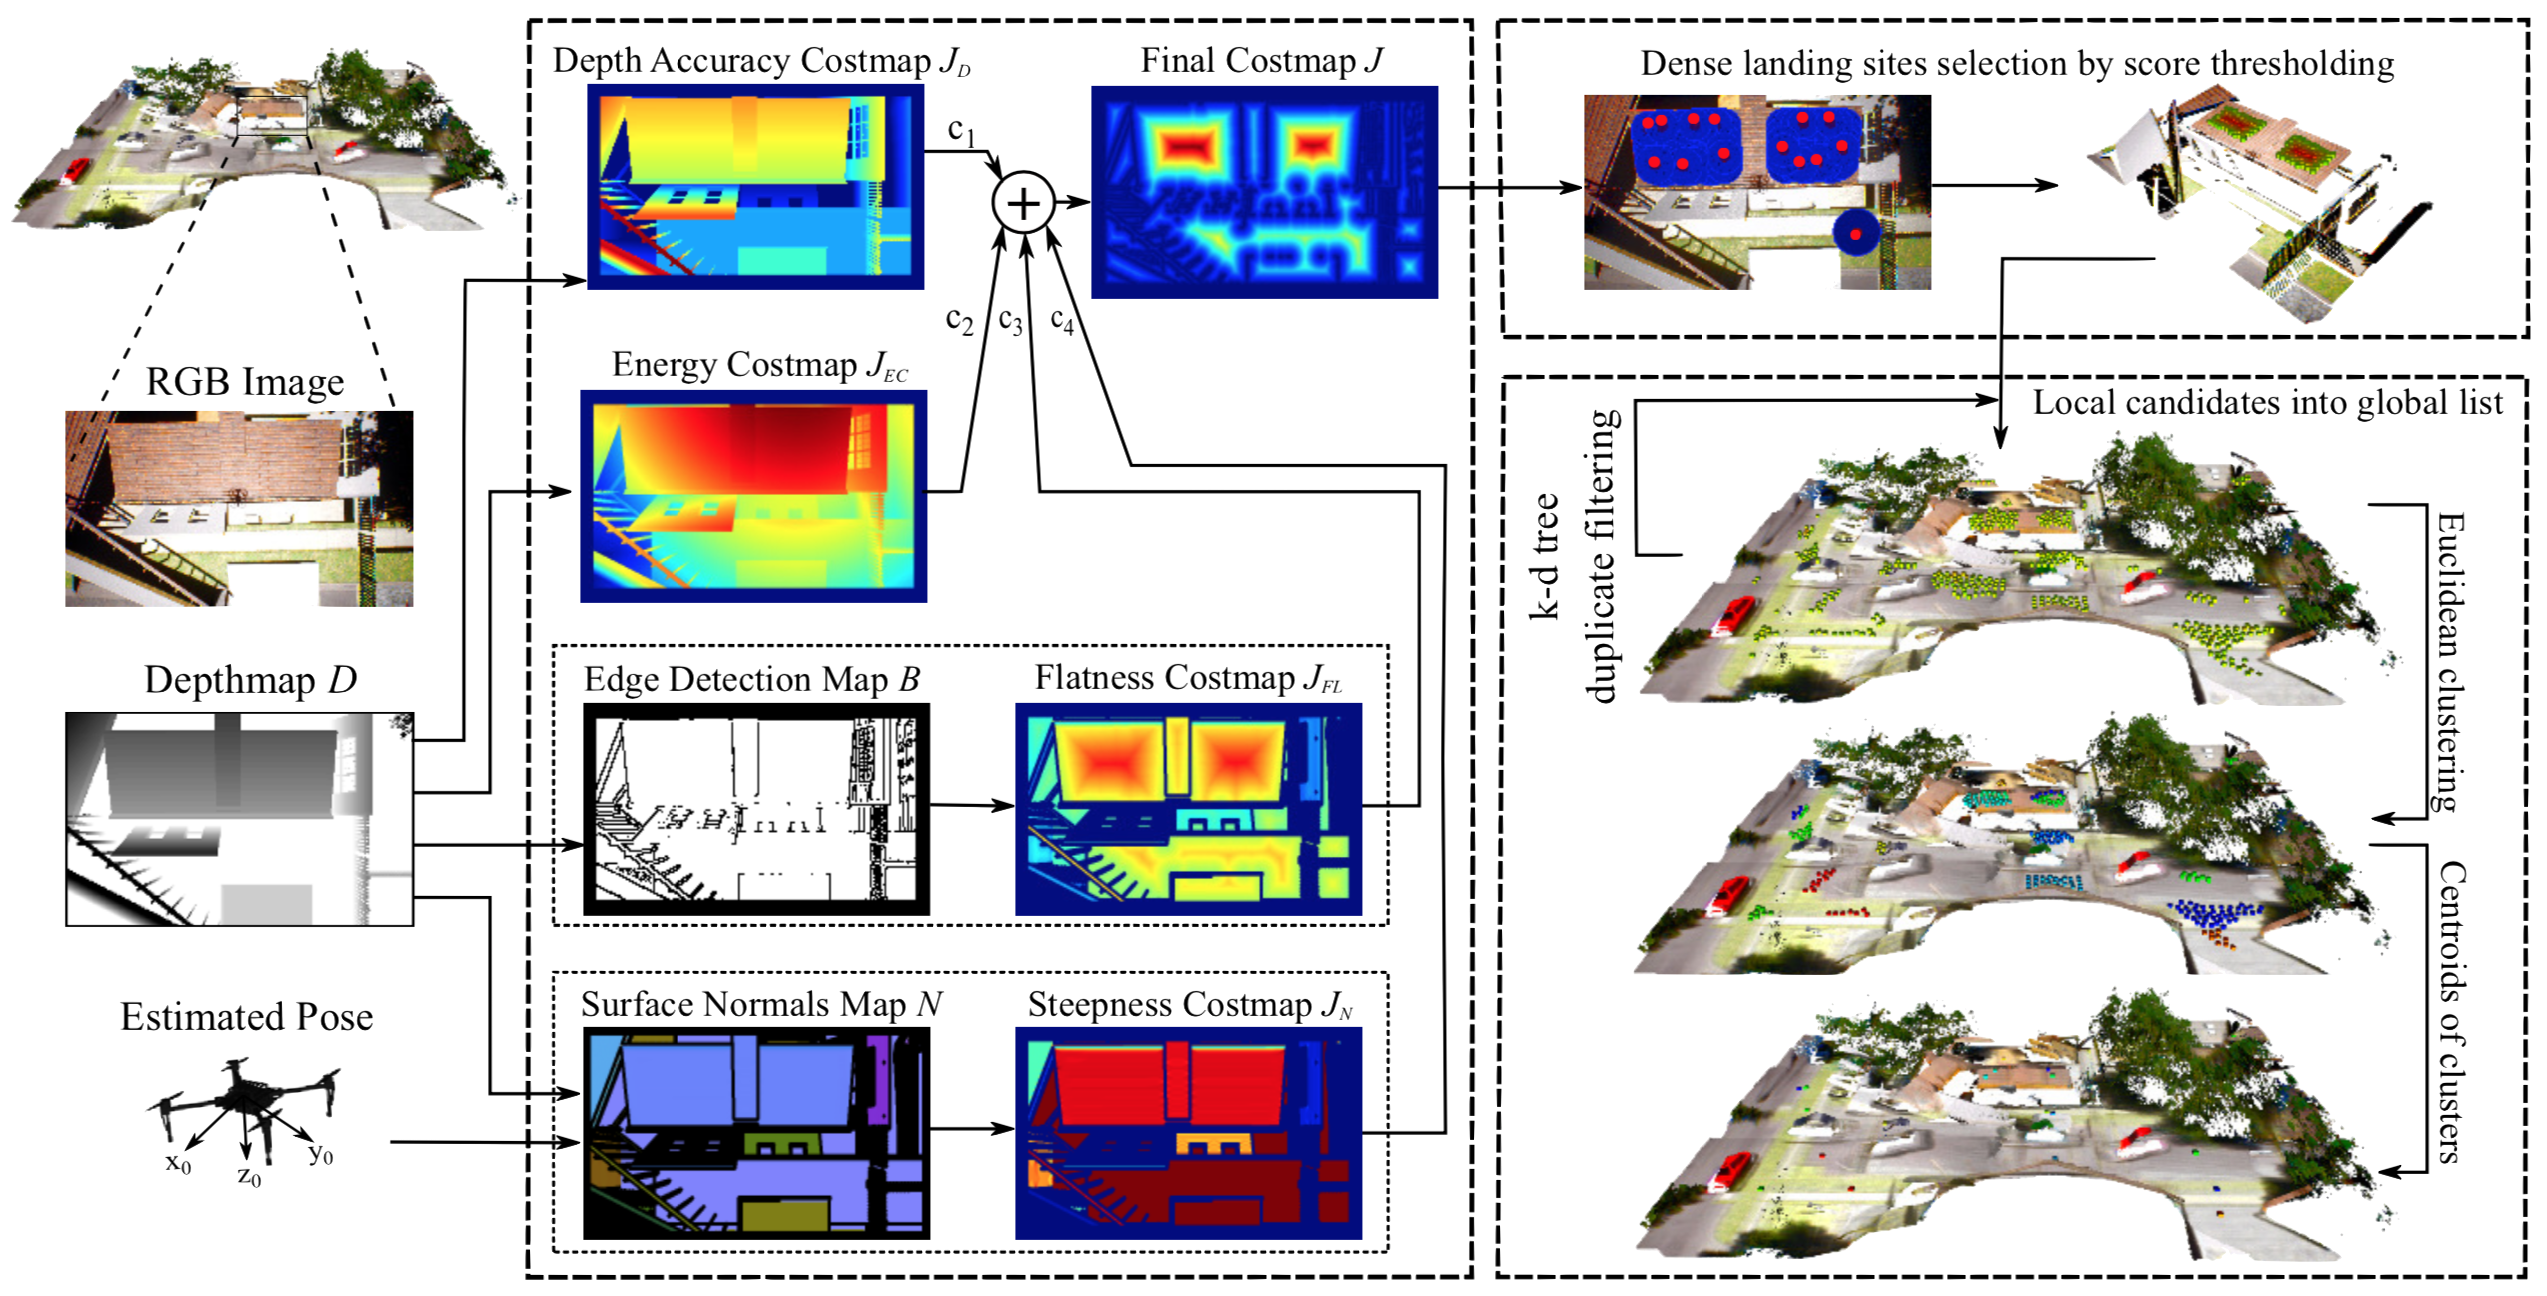
\includegraphics[width=\textwidth]{images/Fig3.png}
        \end{figure}
    \end{frame}

    \begin{frame}{Technical Approach: 3D Volumetric Mapping}
        Probabilistic volumetric map:
        \begin{itemize}
            \item navigation and planning
            \item low-resolution map ($0.5$m) using \textbf{OctoMaps}
            \item faster trajectory planning
        \end{itemize}

        3D textured mesh:
        \begin{itemize}
            \item dynamic map growing using \textbf{Voxblox}
            \item high-resolution mesh transmitted to the rescue team
        \end{itemize}
    \end{frame}

    \begin{frame}{Technical Approach: Landing Trajectory Estimation}
        Minimum-jerk trajectory generator with non-linear optimization:
        \begin{columns}[c,onlytextwidth]
            \column{0.5\textwidth}
                \justifying
                \begin{itemize}
                    \item \textbf{RRT*} for collision free path
                    \item line-of-sight for waypoints
                    \item minimum-snap polynomial trajectories using
                        differential flat model
                    \item high speed arcs in obstacles free regions
                    \item low velocities in tight places
                \end{itemize}
                %Guarantees high speed arcs in obstacles free regions and low
                %velocities in tight places.
            \column{0.5\textwidth}
                \begin{figure}
                    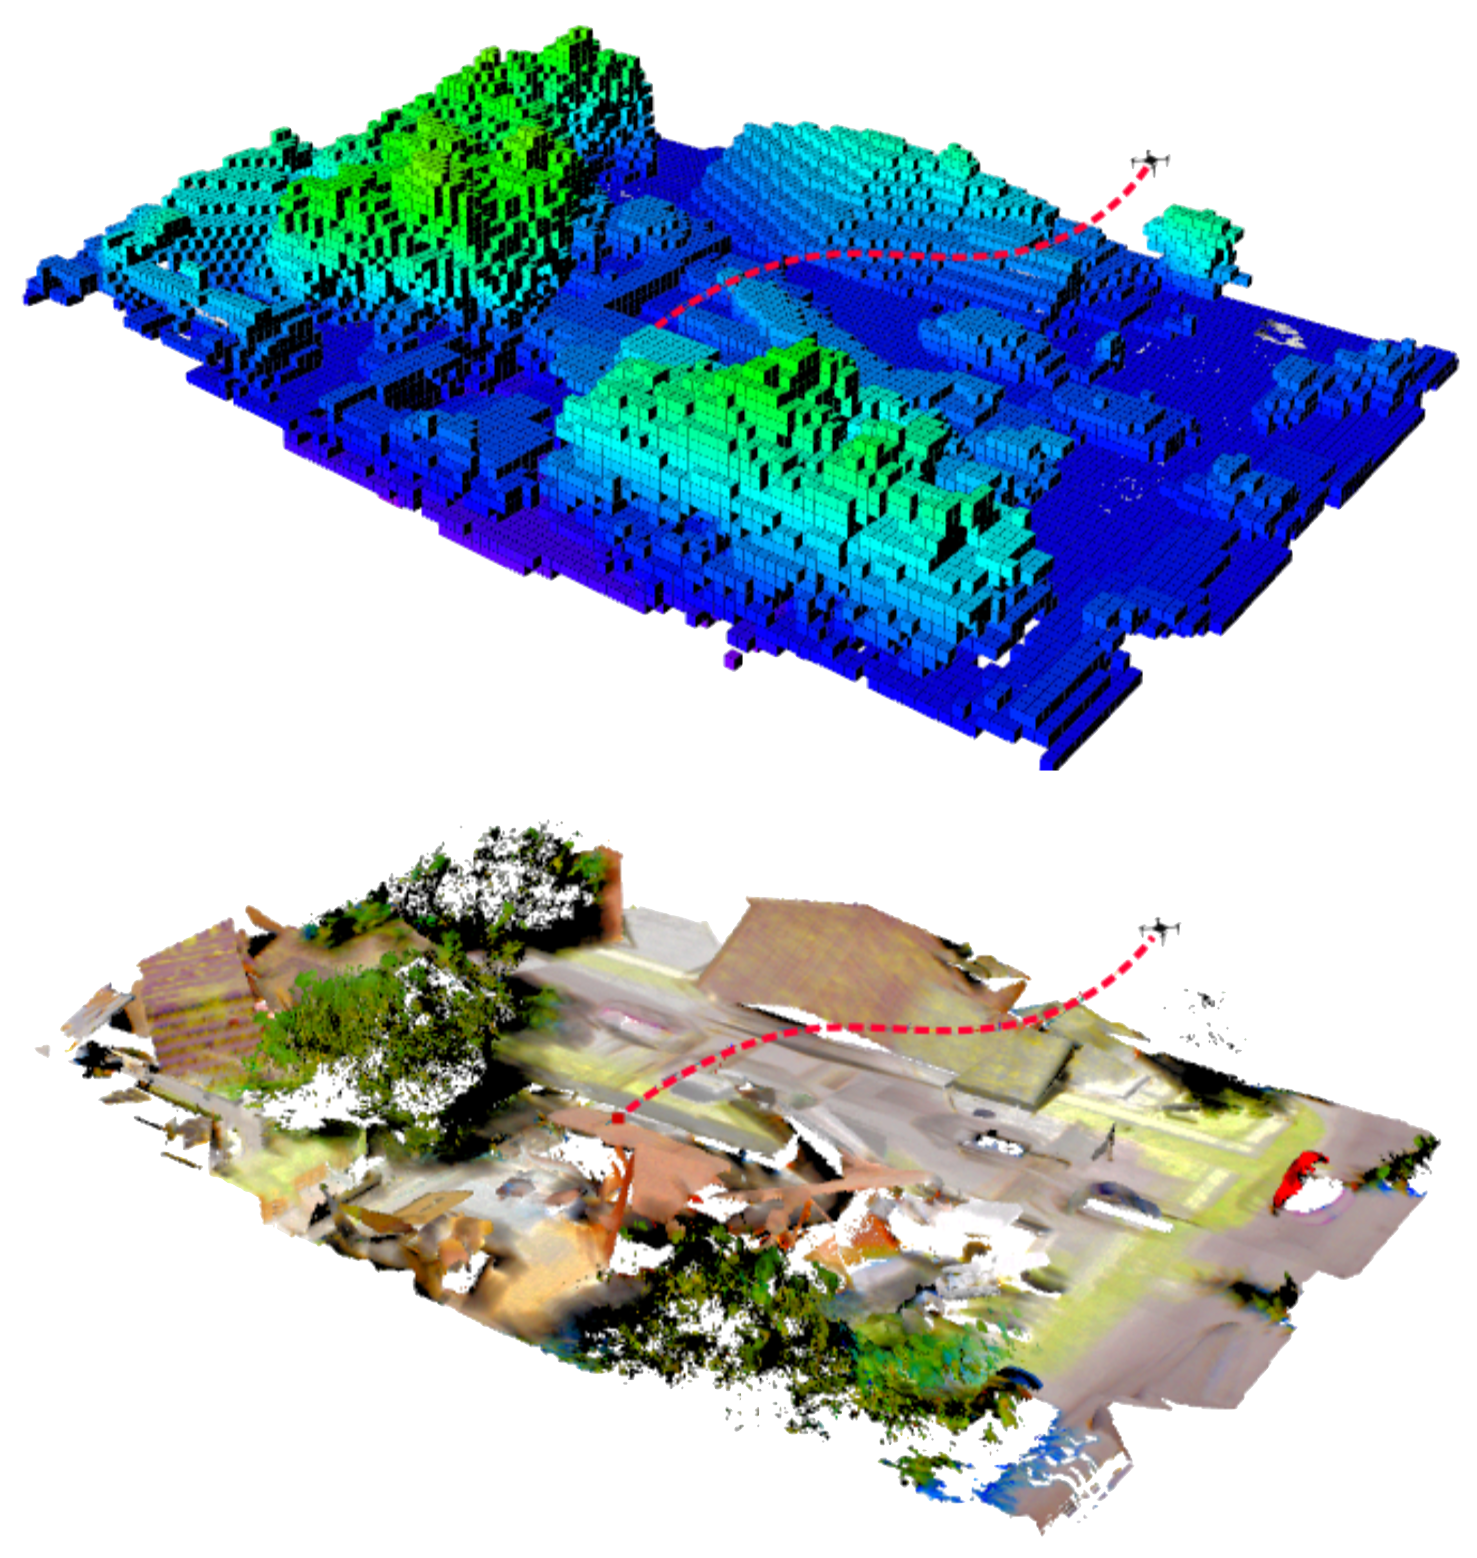
\includegraphics[width=\textwidth]{images/Fig4.png}
                \end{figure}
        \end{columns}
    \end{frame}

%    \begin{frame}{Experimental Evaluation}
%        \begin{figure}%[ht]
%            \begin{minipage}{0.475\linewidth}
%                \centering
%                \textbf{Hyperrealistic Simulation}
%                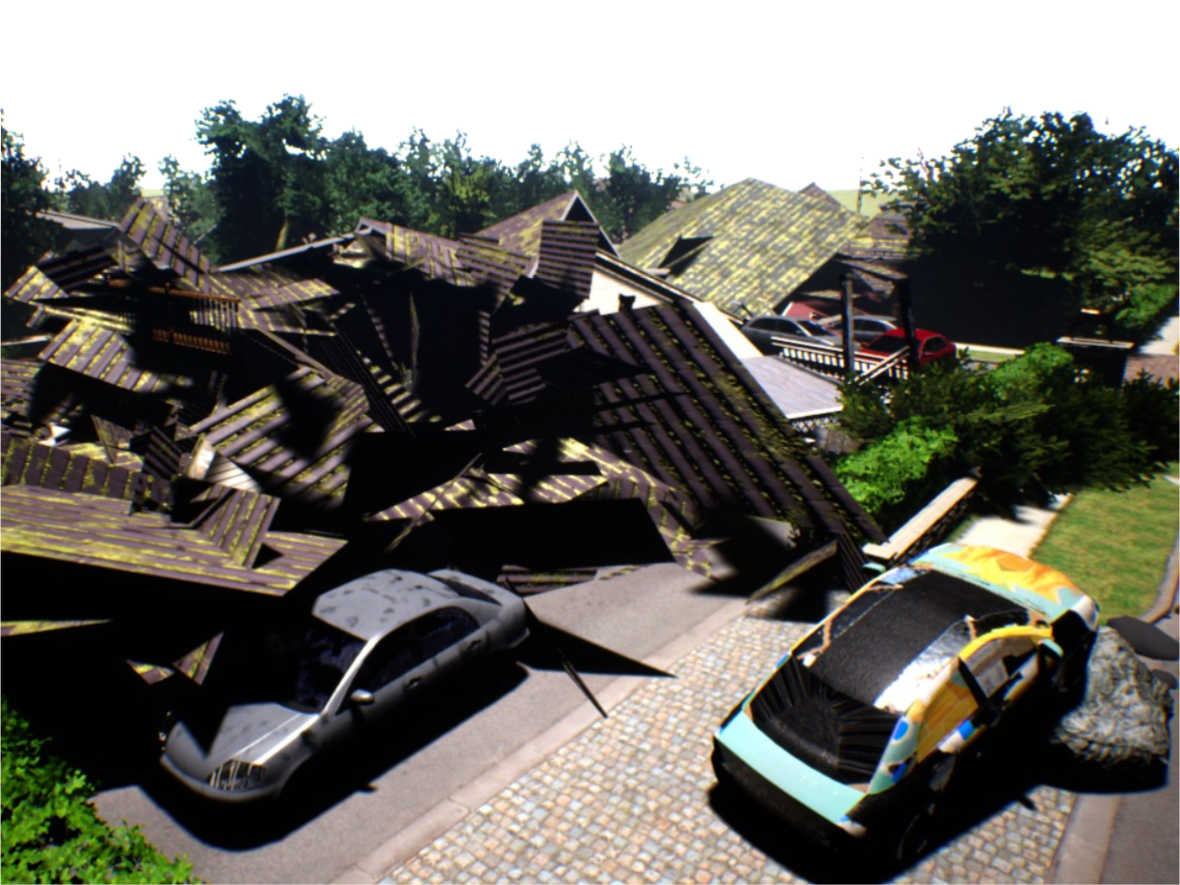
\includegraphics[width=\textwidth]{images/Fig5a.png}
%                \vspace{-0.25cm}
%                {
%                    \scriptsize
%                    \begin{itemize}
%                        \item AirSim + Unreal Engine + ROS
%                        \item RGBD 640x480 20Hz
%                        \item Octomap 0.5m
%                        \item Voxblox 0.1m
%                    \end{itemize}
%                    \vspace{-0.15cm}
%                    %$c_1=0.05, c_2=0.4, c_3=0.4, c_4=0.15$
%                }
%            \end{minipage}
%            \hspace{0.2cm}
%            \begin{minipage}{0.475\linewidth}
%                \centering
%                \textbf{Training Center for Rescue}
%                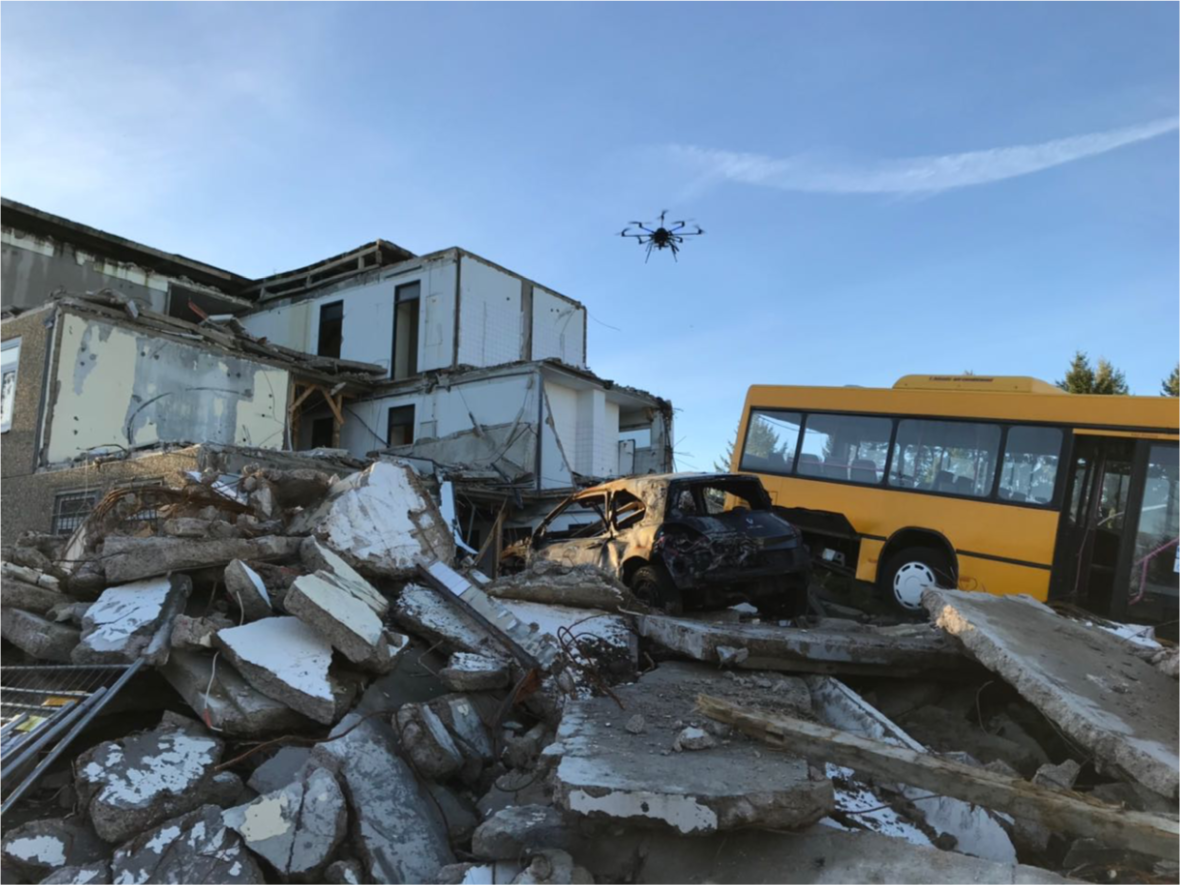
\includegraphics[width=\textwidth]{images/Fig5b.png}
%                \vspace{-0.25cm}
%                {
%                    \scriptsize
%                    \begin{itemize}
%                        \item DJI M100 + NVIDIA TX2
%                        \item ZED stereo camera 640x480 20Hz
%                        \item Octomap 0.5m
%                        \item Voxblox 0.1m
%                    \end{itemize}
%                    \vspace{-0.15cm}
%                    %$c_1=0.15, c_2=0.35, c_3=0.4, c_4=0.1$
%                }
%            \end{minipage}
%        \end{figure}
%    \end{frame}

    \begin{frame}{Experimental Evaluation}
        \begin{figure}
            \caption{
                \justifying
                Costmap evaluation and dense landing sites detection steps
                in both simulated and real-world scenarios.}
            \vspace{-0.3cm}
            \includegraphics[width=\textwidth]{images/Fig6.png}
        \end{figure}
    \end{frame}

%    \begin{frame}{Computation Costs}
%        \begin{columns}[c,onlytextwidth]
%            \column{0.5\textwidth}
%                \begin{itemize}
%                    \item landing site detection algorithm runs in
%                        \textbf{167.5ms} using \textbf{193.8MB}
%                    \item $J_{DE}$, $J_N$, $J_{EC}$ are linear
%                    \item $J_{FL}$ depends on distance transformation
%                        operation: $O(dk)$, $d=2$
%                    \item clustering time and memory complexity:
%                        $O(n^2)$ and $O(n)$
%                \end{itemize}
%
%            \column{0.5\textwidth}
%                \vspace{0.4cm}
%                \begin{figure}
%                    \centering
%                    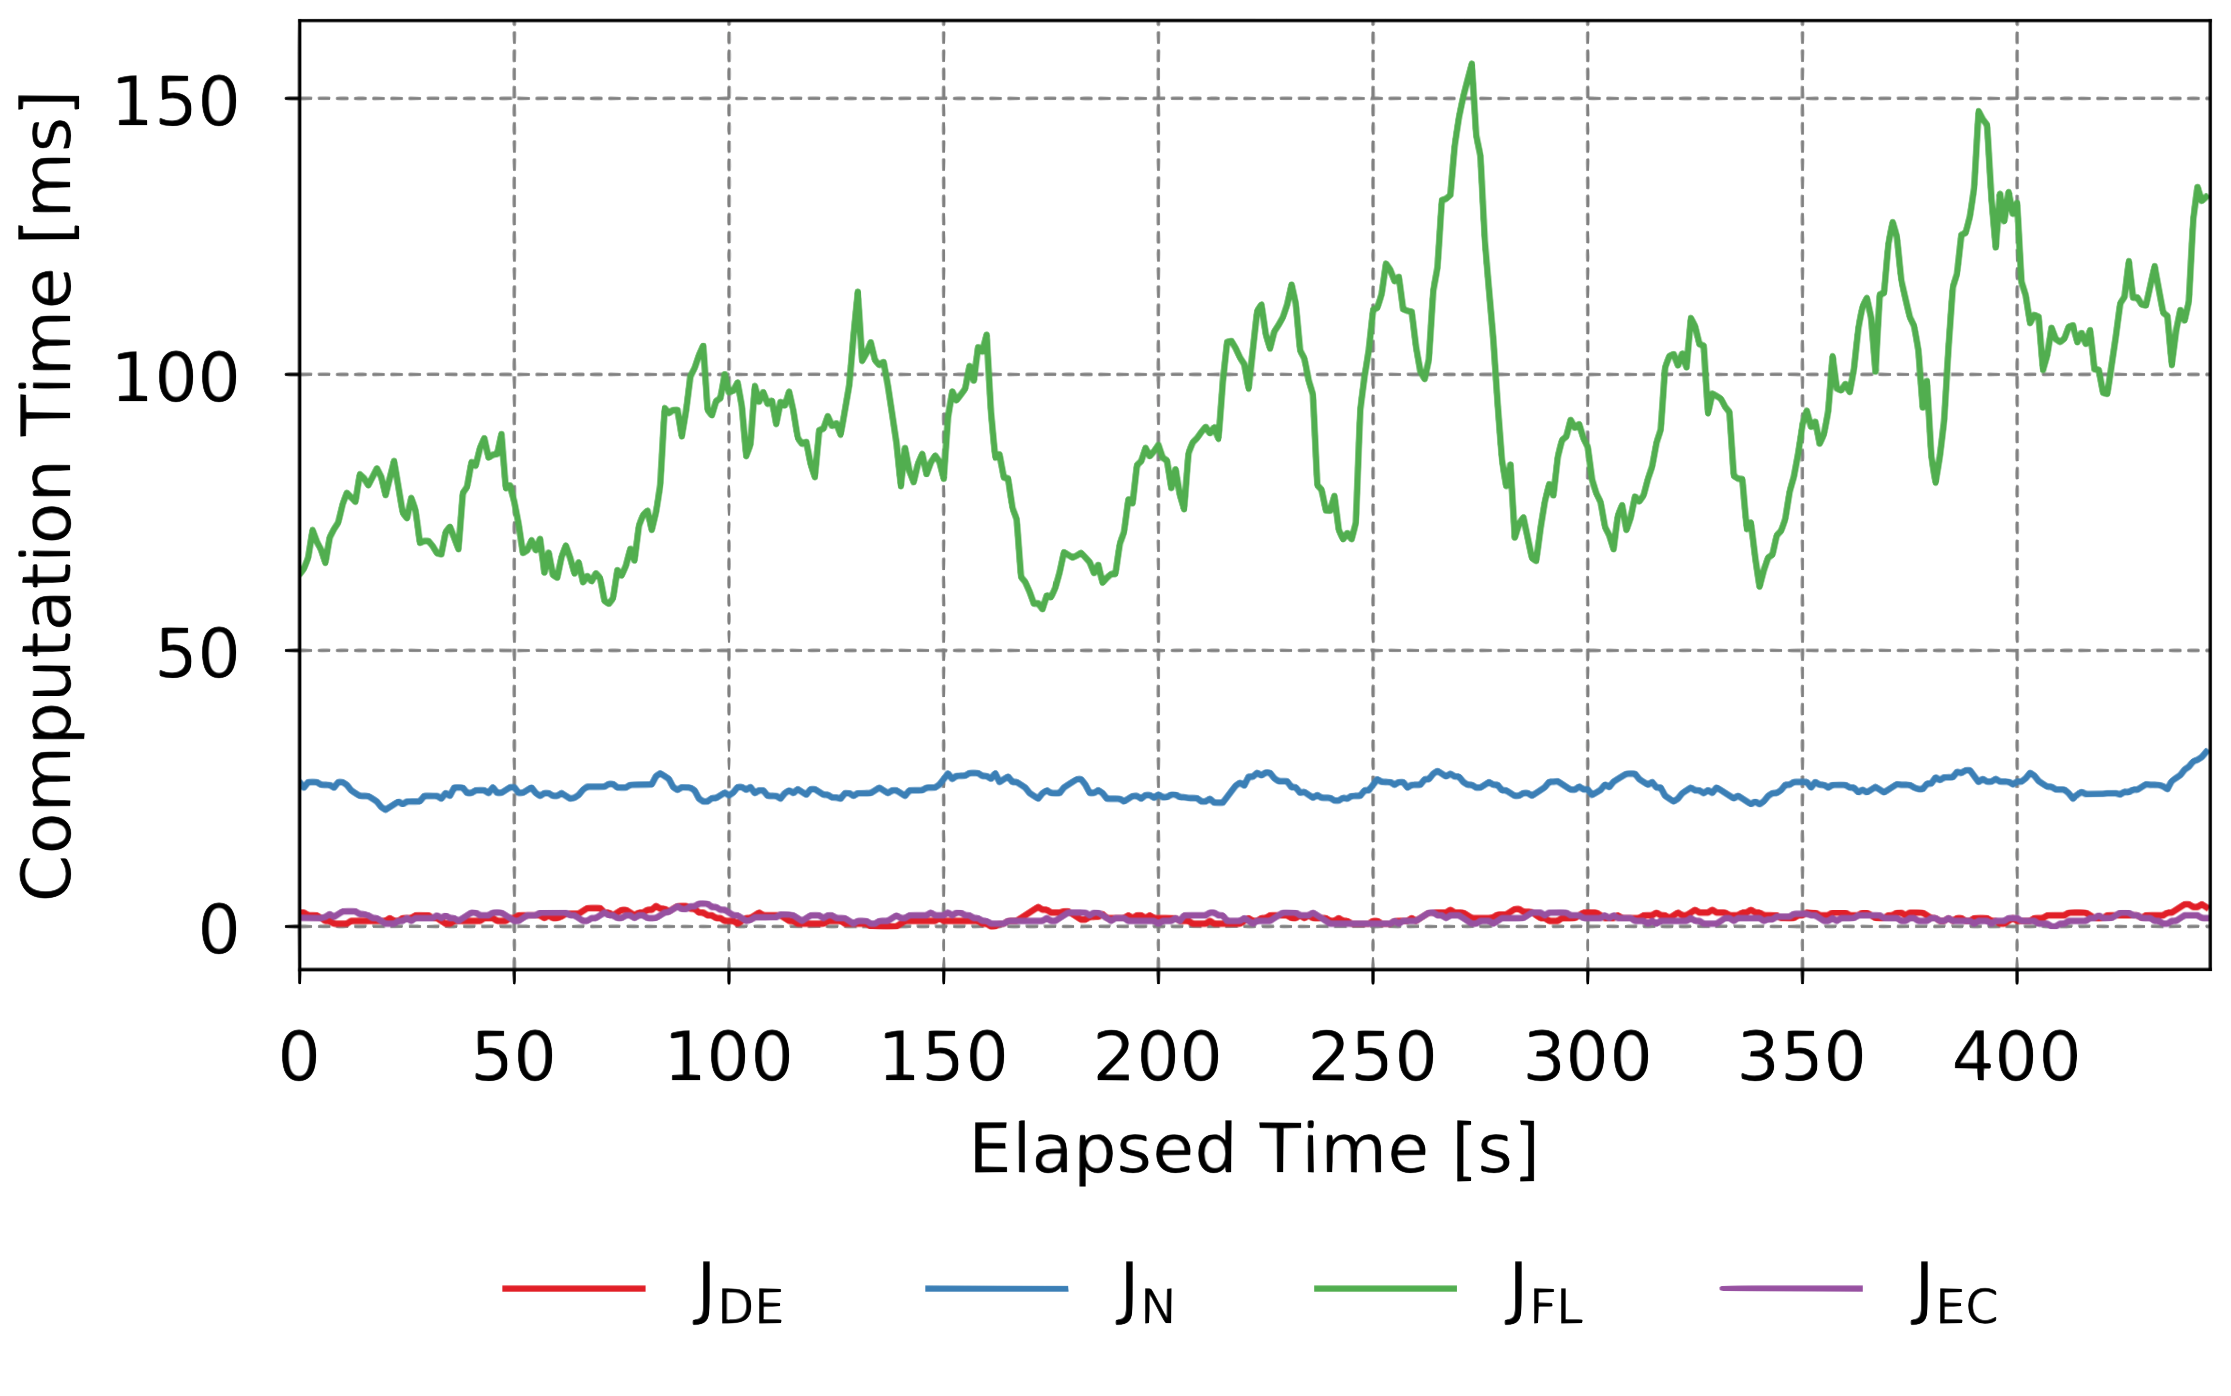
\includegraphics[width=\textwidth]{images/Fig8a.png}
%                \end{figure}
%                \vspace{-0.8cm}
%                \begin{figure}
%                    \centering
%                    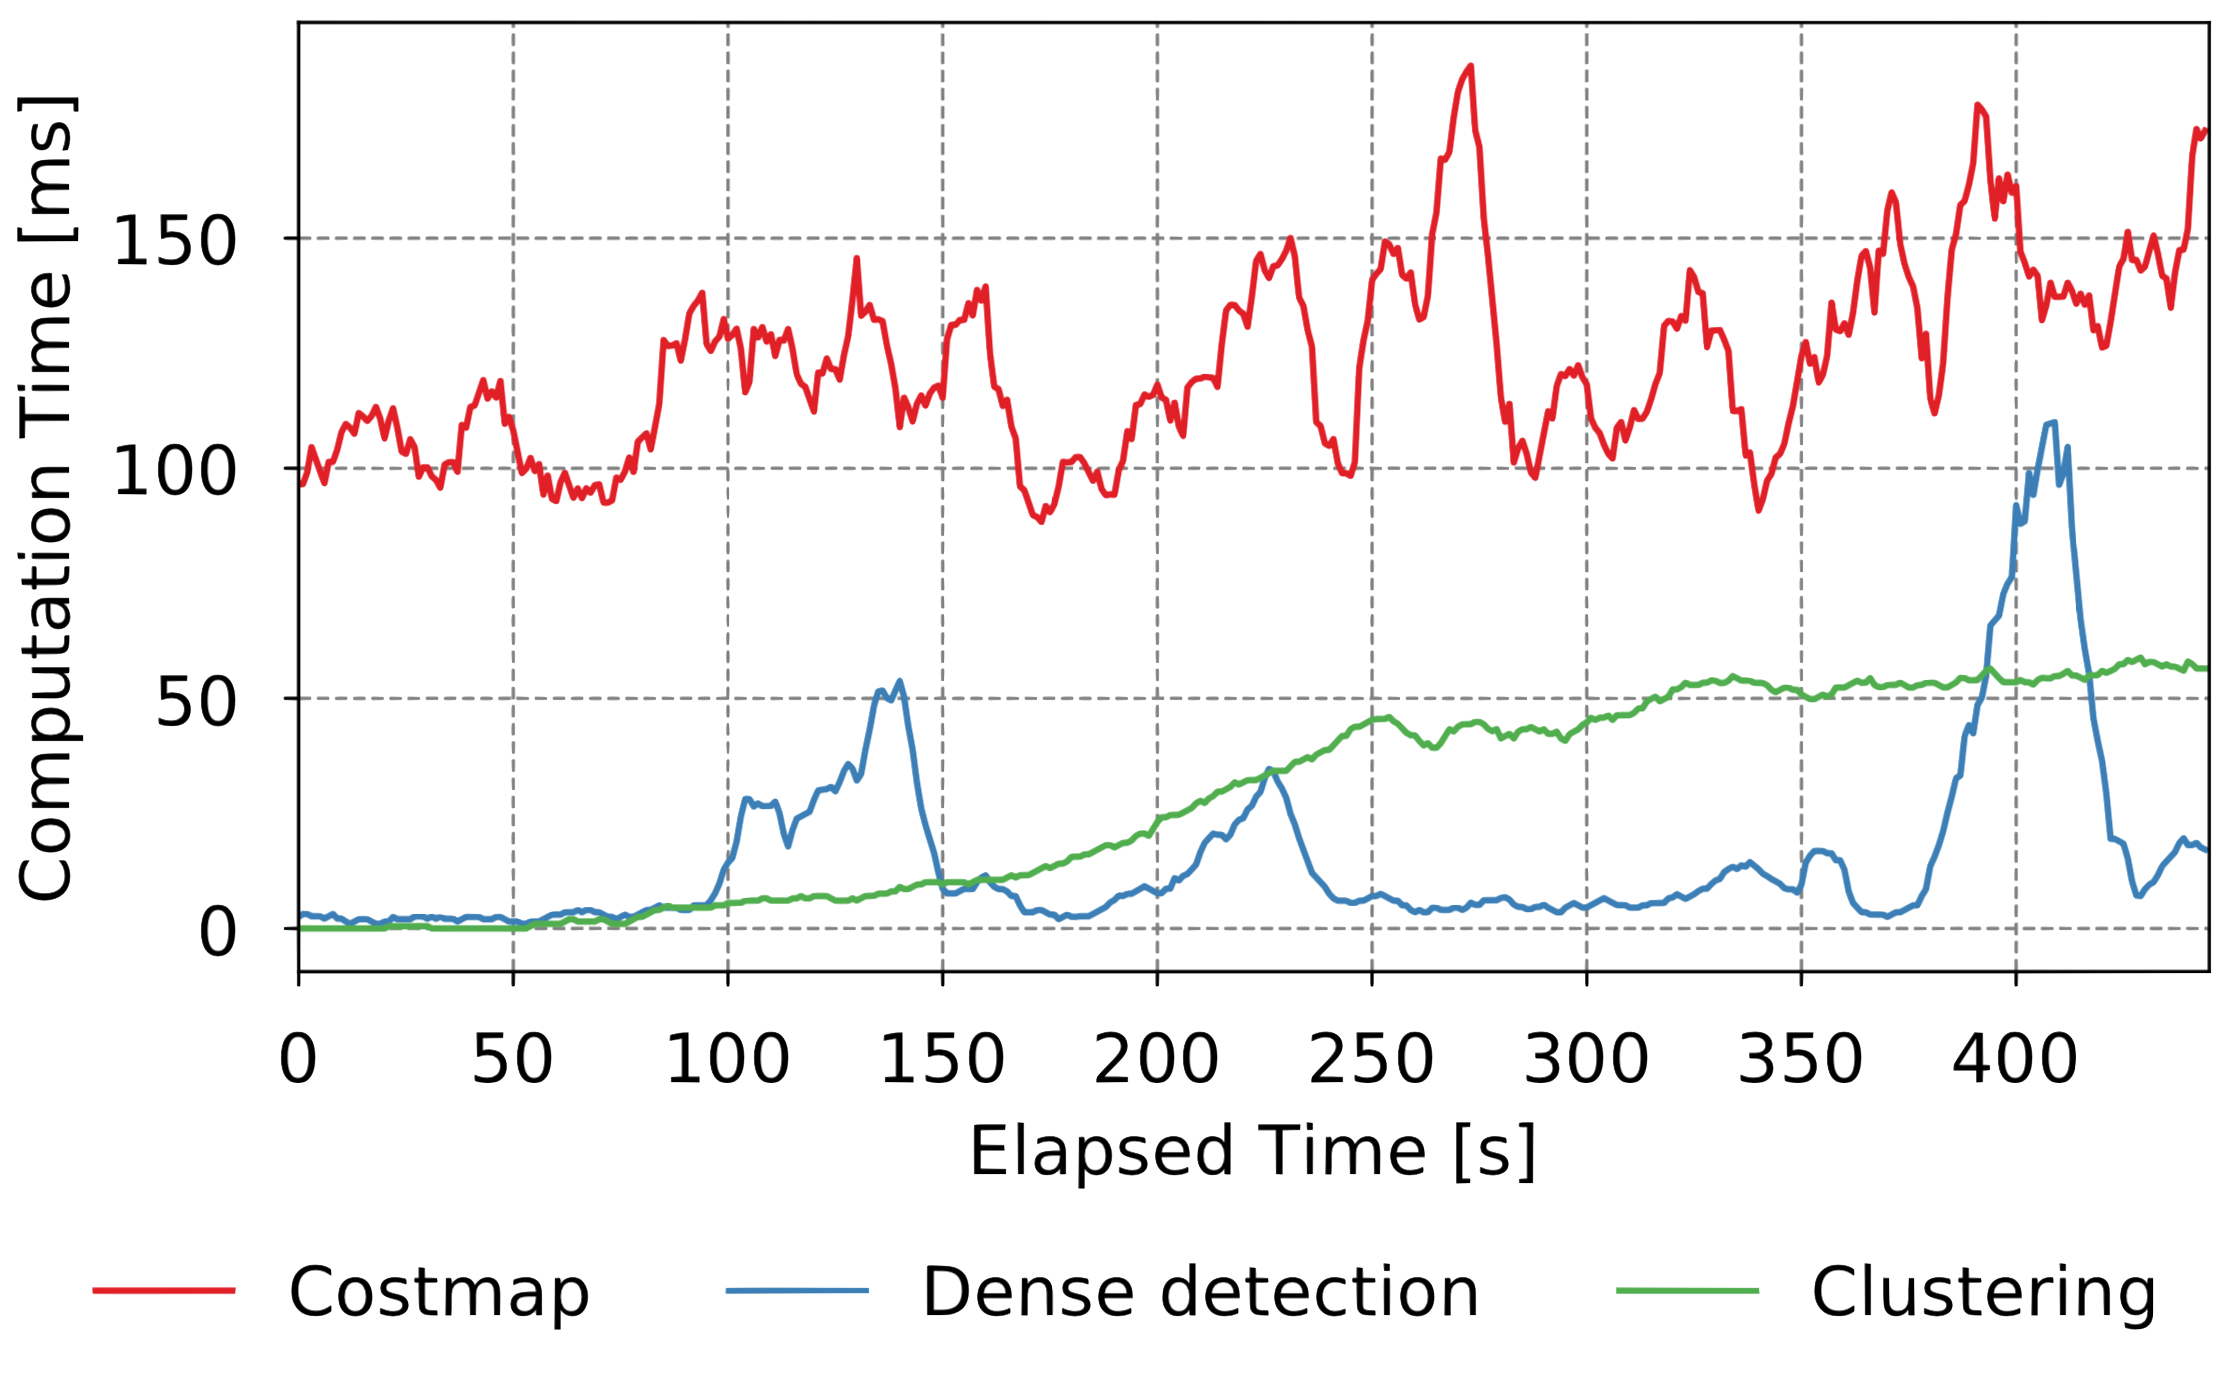
\includegraphics[width=\textwidth]{images/Fig8b.png}
%                \end{figure}
%        \end{columns}
%    \end{frame}

    \begin{frame}{Conclusion}
        \begin{itemize}
            \item \textbf{vision-based autonomous landing system} for UAVs
            \item bioradars, search and rescue operations
            \item hazardous terrain factors
            \item nearest neighbor filtering and clustering
            \item both low and high resolution map
        \end{itemize}
    \end{frame}

    \begin{frame}[standout]
        Q\&A
    \end{frame}

    \appendix

    \begin{frame}{References}
        \bibliography{bibliography}
        \bibliographystyle{ieeetr}
    \end{frame}

\end{document}
